\documentclass[showpacs, preprintnumbers, pra, superscriptaddress, floatfix, onecolumn, longbibliography]{revtex4-1}
\usepackage{amssymb}
\usepackage{amsmath}
\usepackage{float}
\usepackage{graphicx}
\usepackage{epsfig}
\usepackage[T1]{fontenc}
\usepackage{color}


\usepackage[utf8]{inputenc}
%\topmargin=0.2cm

\newcommand{\beq}{\begin{equation}}
\newcommand{\eeq}{\end{equation}}
\newcommand{\bea}{\begin{eqnarray}}
\newcommand{\eea}{\end{eqnarray}}
\newcommand{\nn}{\nonumber}
\newcommand{\no}{\noindent}
\newcommand{\hs}{\hspace{0.1cm}}
\newcommand{\spz}{\hspace{0.7cm}}
\newcommand{\st}{\stackrel}
\newcommand{\eps}{\epsilon}
\newcommand{\veps}{\varepsilon}
\newcommand{\al}{\alpha}
\newcommand{\s}{\sigma}
\newcommand{\lam}{\lambda}
\newcommand{\om}{\omega}
\newcommand{\iom}{i\omega_n}
\newcommand{\de}{\delta}
\newcommand{\D}{\Delta}
\newcommand{\goto}{\rightarrow}
\newcommand{\lab}{\label}
\newcommand{\be}{\beta}
\newcommand{\zb}{\bar{z}}
\newcommand{\p}{\partial}\newcommand{\vp}{\varphi}
\newcommand{\ra}{\rangle}
\newcommand{\la}{\langle}
\newcommand{\Ga}{\Gamma}
\newcommand{\ga}{\gamma}
\newcommand{\app}{\approx}
\newcommand{\ua}{\uparrow}
\newcommand{\da}{\downarrow}
\newcommand{\Ua}{\Uparrow}
\newcommand{\Da}{\Downarrow}
\newcommand{\dmi}{\frac{1}{2}}
\newcommand{\lra}{\longrightarrow}
\newcommand{\Lra}{\Leftrightarrow}
\newcommand{\tht}{\theta}
\newcommand{\pbf}{}
\newcommand{\SM}{S}
\newcommand{\uul}[1] {\underline{\underline{ #1}}}
\def\mean#1{\left< #1 \right>}

\begin{document}

\title{}


\maketitle

\section{Details of the density-functional (DFT) calculations}

All DFT-based results of this work are obtained with a calculation of a MnBi$_4$Te$_7$ slab made of eight blocks (i.e. four septuple layers and four quintuple layers) and of a vacuum of 30 Bohr. We use the experimental lattice parameters.

\section{Surface state angular momentum reversal within DFT}
\begin{figure*}[h!]
 \centering
 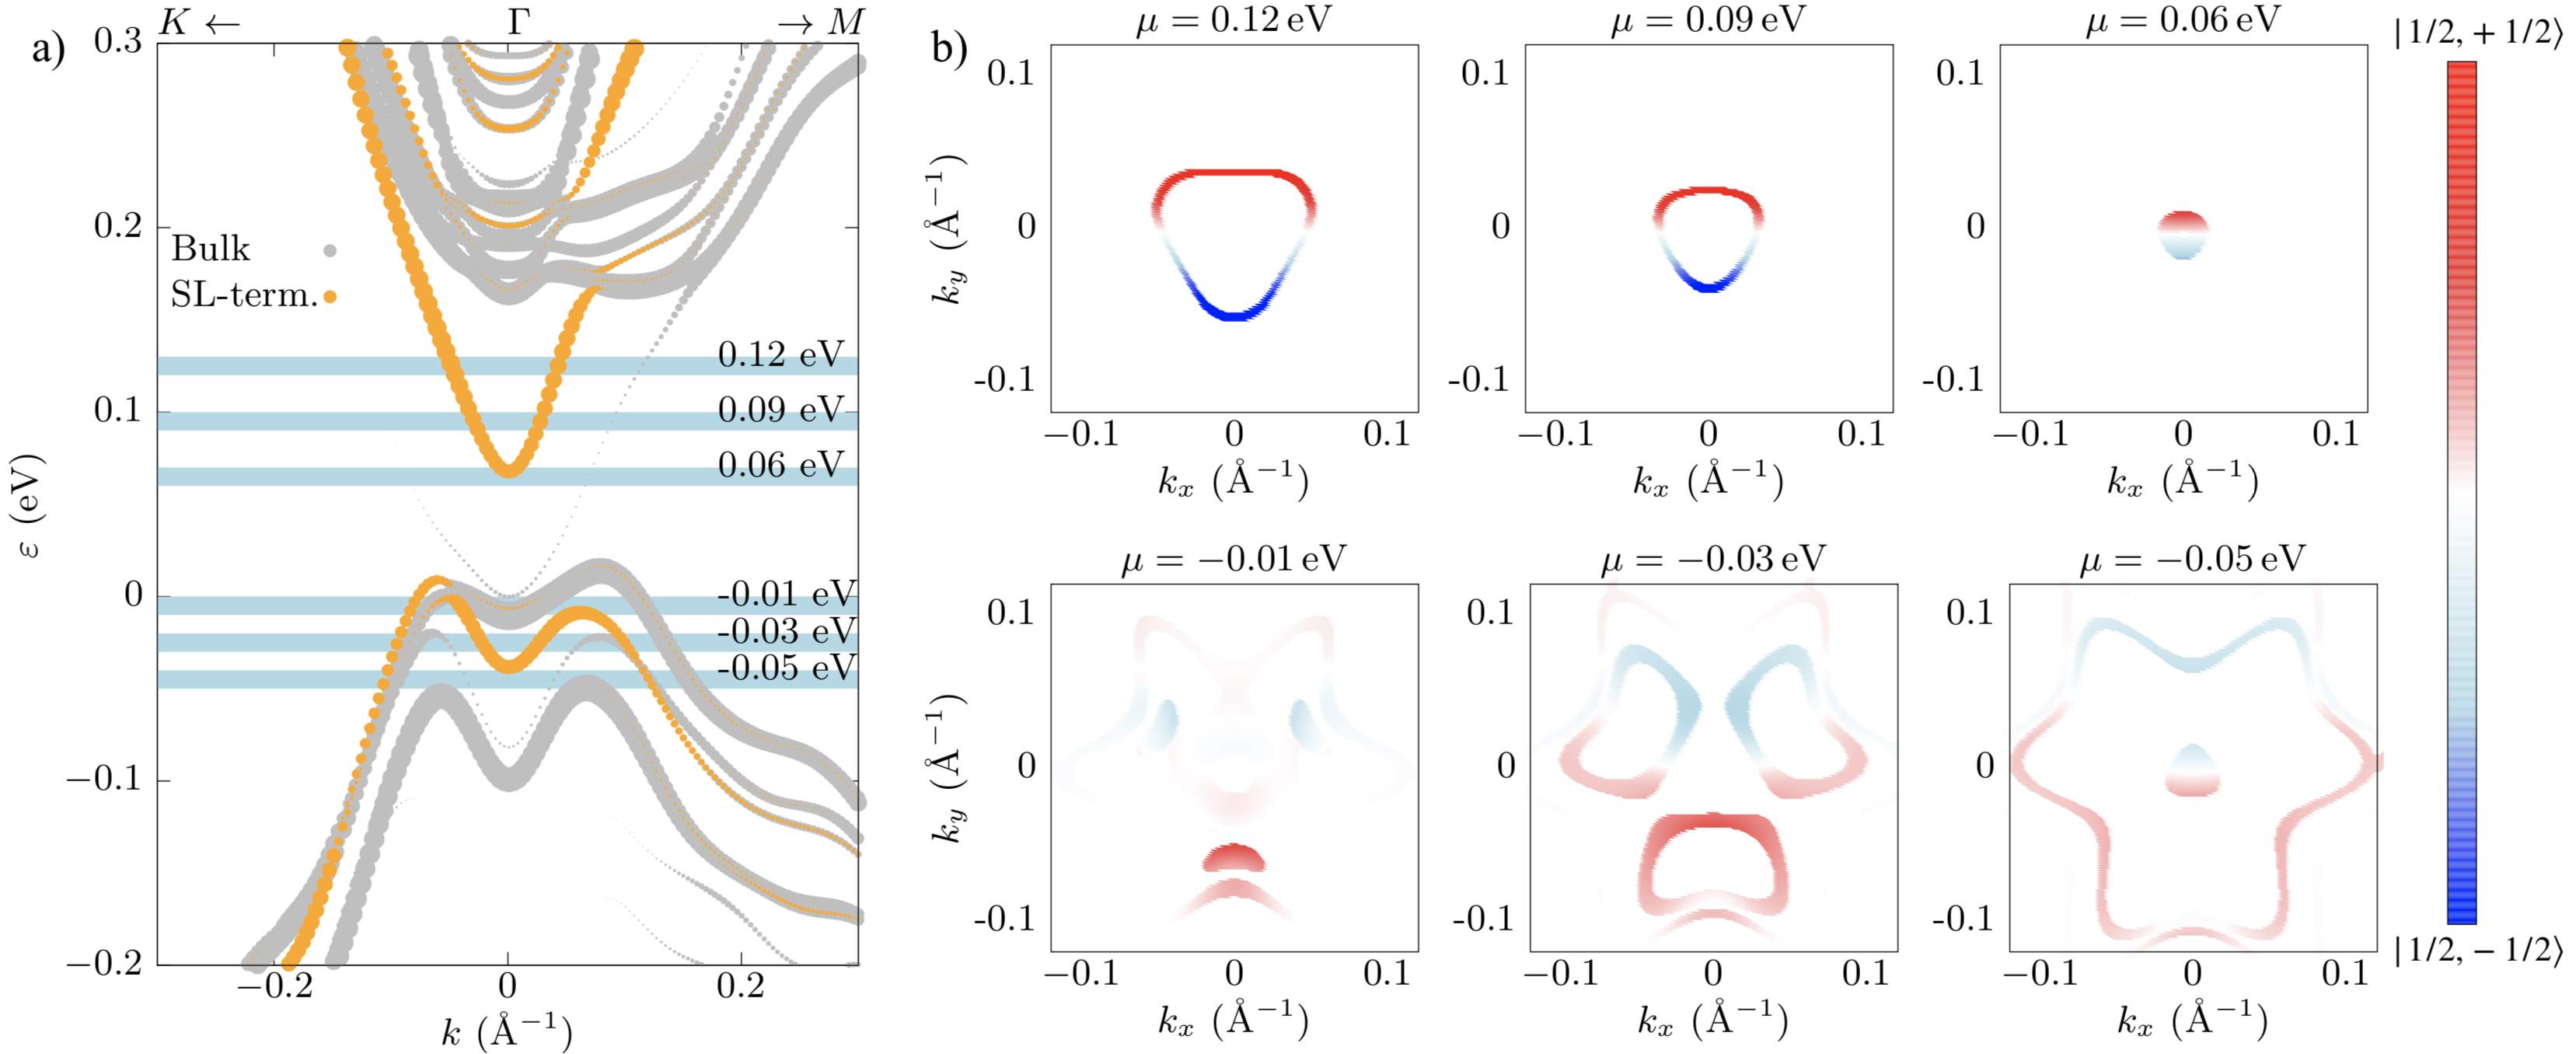
\includegraphics[width=18 cm]{sl.png}
	\caption{a) MnBi$_4$Te$_7$ band structure projected on the outmost septuple layer (SL-term.) and on the four inner blocks (Bulk). 
	b): Constant energy contours of septuple layer-projected band-structure. In this projection, for simplicity we only consider the Bi or Te states with $J=1/2$, which we found to dominate the upper part of the Dirac cone.
	}
	\label{dft_sl}
\end{figure*}


\bibliography{ref}
\end{document}


